\documentclass[11pt,preprint]{elsarticle}

\usepackage{lmodern}
%%%% My spacing
\usepackage{setspace}
\setstretch{1.2}
\DeclareMathSizes{12}{14}{10}{10}

% Wrap around which gives all figures included the [H] command, or places it "here". This can be tedious to code in Rmarkdown.
\usepackage{float}
\let\origfigure\figure
\let\endorigfigure\endfigure
\renewenvironment{figure}[1][2] {
    \expandafter\origfigure\expandafter[H]
} {
    \endorigfigure
}

\let\origtable\table
\let\endorigtable\endtable
\renewenvironment{table}[1][2] {
    \expandafter\origtable\expandafter[H]
} {
    \endorigtable
}


\usepackage{ifxetex,ifluatex}
\usepackage{fixltx2e} % provides \textsubscript
\ifnum 0\ifxetex 1\fi\ifluatex 1\fi=0 % if pdftex
  \usepackage[T1]{fontenc}
  \usepackage[utf8]{inputenc}
\else % if luatex or xelatex
  \ifxetex
    \usepackage{mathspec}
    \usepackage{xltxtra,xunicode}
  \else
    \usepackage{fontspec}
  \fi
  \defaultfontfeatures{Mapping=tex-text,Scale=MatchLowercase}
  \newcommand{\euro}{€}
\fi

\usepackage{amssymb, amsmath, amsthm, amsfonts}

\def\bibsection{\section*{References}} %%% Make "References" appear before bibliography


\usepackage[numbers]{natbib}

\usepackage{longtable}
\usepackage[margin=2.3cm,bottom=2cm,top=2.5cm, includefoot]{geometry}
\usepackage{fancyhdr}
\usepackage[bottom, hang, flushmargin]{footmisc}
\usepackage{graphicx}
\numberwithin{equation}{section}
\numberwithin{figure}{section}
\numberwithin{table}{section}
\setlength{\parindent}{0cm}
\setlength{\parskip}{1.3ex plus 0.5ex minus 0.3ex}
\usepackage{textcomp}
\renewcommand{\headrulewidth}{0.2pt}
\renewcommand{\footrulewidth}{0.3pt}

\usepackage{array}
\newcolumntype{x}[1]{>{\centering\arraybackslash\hspace{0pt}}p{#1}}

%%%%  Remove the "preprint submitted to" part. Don't worry about this either, it just looks better without it:
\makeatletter
\def\ps@pprintTitle{%
  \let\@oddhead\@empty
  \let\@evenhead\@empty
  \let\@oddfoot\@empty
  \let\@evenfoot\@oddfoot
}
\makeatother

 \def\tightlist{} % This allows for subbullets!

\usepackage{hyperref}
\hypersetup{breaklinks=true,
            bookmarks=true,
            colorlinks=true,
            citecolor=blue,
            urlcolor=blue,
            linkcolor=blue,
            pdfborder={0 0 0}}


% The following packages allow huxtable to work:
\usepackage{siunitx}
\usepackage{multirow}
\usepackage{hhline}
\usepackage{calc}
\usepackage{tabularx}
\usepackage{booktabs}
\usepackage{caption}


\newenvironment{columns}[1][]{}{}

\newenvironment{column}[1]{\begin{minipage}{#1}\ignorespaces}{%
\end{minipage}
\ifhmode\unskip\fi
\aftergroup\useignorespacesandallpars}

\def\useignorespacesandallpars#1\ignorespaces\fi{%
#1\fi\ignorespacesandallpars}

\makeatletter
\def\ignorespacesandallpars{%
  \@ifnextchar\par
    {\expandafter\ignorespacesandallpars\@gobble}%
    {}%
}
\makeatother


% definitions for citeproc citations
\NewDocumentCommand\citeproctext{}{}
\NewDocumentCommand\citeproc{mm}{%
\href{\#cite.\detokenize{#1}}{#2}\nocite{#1}}

\makeatletter
% allow citations to break across lines
\let\@cite@ofmt\@firstofone
% avoid brackets around text for \cite:
\def\@biblabel#1{}
\def\@cite#1#2{{#1\if@tempswa , #2\fi}}
\makeatother
\newlength{\cslhangindent}
\setlength{\cslhangindent}{1.5em}
\newlength{\csllabelwidth}
\setlength{\csllabelwidth}{3em}
\newenvironment{CSLReferences}[2] % #1 hanging-indent, #2 entry-spacing
{\begin{list}{}{%
	\setlength{\itemindent}{0pt}
	\setlength{\leftmargin}{0pt}
	\setlength{\parsep}{0pt}
	% turn on hanging indent if param 1 is 1
	\ifodd #1
	\setlength{\leftmargin}{\cslhangindent}
	\setlength{\itemindent}{-1\cslhangindent}
	\fi
	% set entry spacing
	\setlength{\itemsep}{#2\baselineskip}}}
{\end{list}}

\usepackage{calc}
\newcommand{\CSLBlock}[1]{\hfill\break\parbox[t]{\linewidth}{\strut\ignorespaces#1\strut}}
\newcommand{\CSLLeftMargin}[1]{\parbox[t]{\csllabelwidth}{\strut#1\strut}}
\newcommand{\CSLRightInline}[1]{\parbox[t]{\linewidth - \csllabelwidth}{\strut#1\strut}}
\newcommand{\CSLIndent}[1]{\hspace{\cslhangindent}#1}


\urlstyle{same}  % don't use monospace font for urls
\setlength{\parindent}{0pt}
\setlength{\parskip}{6pt plus 2pt minus 1pt}
\setlength{\emergencystretch}{3em}  % prevent overfull lines
\setcounter{secnumdepth}{5}

%%% Use protect on footnotes to avoid problems with footnotes in titles
\let\rmarkdownfootnote\footnote%
\def\footnote{\protect\rmarkdownfootnote}
\IfFileExists{upquote.sty}{\usepackage{upquote}}{}

%%% Include extra packages specified by user

%%% Hard setting column skips for reports - this ensures greater consistency and control over the length settings in the document.
%% page layout
%% paragraphs
\setlength{\baselineskip}{12pt plus 0pt minus 0pt}
\setlength{\parskip}{12pt plus 0pt minus 0pt}
\setlength{\parindent}{0pt plus 0pt minus 0pt}
%% floats
\setlength{\floatsep}{12pt plus 0 pt minus 0pt}
\setlength{\textfloatsep}{20pt plus 0pt minus 0pt}
\setlength{\intextsep}{14pt plus 0pt minus 0pt}
\setlength{\dbltextfloatsep}{20pt plus 0pt minus 0pt}
\setlength{\dblfloatsep}{14pt plus 0pt minus 0pt}
%% maths
\setlength{\abovedisplayskip}{12pt plus 0pt minus 0pt}
\setlength{\belowdisplayskip}{12pt plus 0pt minus 0pt}
%% lists
\setlength{\topsep}{10pt plus 0pt minus 0pt}
\setlength{\partopsep}{3pt plus 0pt minus 0pt}
\setlength{\itemsep}{5pt plus 0pt minus 0pt}
\setlength{\labelsep}{8mm plus 0mm minus 0mm}
\setlength{\parsep}{\the\parskip}
\setlength{\listparindent}{\the\parindent}
%% verbatim
\setlength{\fboxsep}{5pt plus 0pt minus 0pt}



\begin{document}



\begin{frontmatter}  %

\title{An analytical briefing on content trends, audience preferences,
and production dynamics}

% Set to FALSE if wanting to remove title (for submission)




\author[Add1]{Linda Dube}
\ead{23084103@sun.ac.za}





\address[Add1]{Stellenbosch University, Western Cape}


\begin{abstract}
\small{
This report explores patterns in Netflix content using crdits, titles
and movie\_infor data, focusing on popularity, content type, country of
origin, and movie characteristics. Findings show that TV shows
consistently outperform movies in popularity, with UK and Sweden leading
in show performance. Meanwhile, the US and Mexico dominate in film
popularity, and India produces the longest movies. These insights offer
strategic direction for content investment in future streaming ventures.
}
\end{abstract}

\vspace{1cm}





\vspace{0.5cm}

\end{frontmatter}

\setcounter{footnote}{0}



%________________________
% Header and Footers
%%%%%%%%%%%%%%%%%%%%%%%%%%%%%%%%%
\pagestyle{fancy}
\chead{}
\rhead{}
\lfoot{}
\rfoot{\footnotesize Page \thepage}
\lhead{}
%\rfoot{\footnotesize Page \thepage } % "e.g. Page 2"
\cfoot{}

%\setlength\headheight{30pt}
%%%%%%%%%%%%%%%%%%%%%%%%%%%%%%%%%
%________________________

\headsep 35pt % So that header does not go over title




\section{\texorpdfstring{Introduction
\label{Introduction}}{Introduction }}\label{introduction}

With Netflix facing a decline in users and share price, understanding
content preferences is critical for new streaming ventures. This
analysis examines content popularity, regional trends, and movie
characteristics on Netflix. By analyzing shows and movies by country,
runtime, and cast structure, we identify patterns in global viewing
behavior. The findings aim to inform investor decisions and optimize
future content strategies.

\section*{Data}\label{data}
\addcontentsline{toc}{section}{Data}

\begin{Shaded}
\begin{Highlighting}[]
\NormalTok{titles }\OtherTok{\textless{}{-}} \FunctionTok{readRDS}\NormalTok{(}\StringTok{"C:/Users/sukol/Documents/Masters frst semester/Data Science Exam/Data{-}Science{-}Exam/23084103\_Datascience\_Exam/Tex\_Ex/23084103\_Exam/Question 3/Tex\_Ex/23084103\_Netflix/data/netflix/titles.rds"}\NormalTok{)}

\NormalTok{credits }\OtherTok{\textless{}{-}} \FunctionTok{readRDS}\NormalTok{(}\StringTok{"C:/Users/sukol/Documents/Masters frst semester/Data Science Exam/Data{-}Science{-}Exam/23084103\_Datascience\_Exam/Tex\_Ex/23084103\_Exam/Question 3/Tex\_Ex/23084103\_Netflix/data/netflix/credits.rds"}\NormalTok{)}
\NormalTok{movie\_Info }\OtherTok{\textless{}{-}} \FunctionTok{read.csv}\NormalTok{(}\StringTok{"C:/Users/sukol/Documents/Masters frst semester/Data Science Exam/Data{-}Science{-}Exam/23084103\_Datascience\_Exam/Tex\_Ex/23084103\_Exam/Question 3/Tex\_Ex/23084103\_Netflix/data/netflix/netflix\_movies.csv"}\NormalTok{)}

\CommentTok{\# Save as CSV}
\FunctionTok{write.csv}\NormalTok{(titles, }\StringTok{"C:/Users/sukol/Documents/titles.csv"}\NormalTok{, }\AttributeTok{row.names =} \ConstantTok{FALSE}\NormalTok{)}
\FunctionTok{write.csv}\NormalTok{(credits, }\StringTok{"C:/Users/sukol/Documents/credits.csv"}\NormalTok{, }\AttributeTok{row.names =} \ConstantTok{FALSE}\NormalTok{)}

\FunctionTok{library}\NormalTok{(summarytools)}
\end{Highlighting}
\end{Shaded}

\begin{verbatim}
## Warning: package 'summarytools' was built under R version 4.4.3
\end{verbatim}

\begin{Shaded}
\begin{Highlighting}[]
\FunctionTok{options}\NormalTok{(}\AttributeTok{summarytools.style =} \StringTok{"plain"}\NormalTok{, }\AttributeTok{summarytools.browser.notknit =} \ConstantTok{FALSE}\NormalTok{)}

\NormalTok{titles\_summary }\OtherTok{\textless{}{-}} \FunctionTok{dfSummary}\NormalTok{(titles, }\AttributeTok{plain.ascii =} \ConstantTok{TRUE}\NormalTok{, }\AttributeTok{style =} \StringTok{"grid"}\NormalTok{)}
\FunctionTok{print}\NormalTok{(titles\_summary)}
\end{Highlighting}
\end{Shaded}

\begin{verbatim}
## Data Frame Summary  
## titles  
## Dimensions: 5806 x 15  
## Duplicates: 0  
## 
## +----+----------------------+-------------------------------+----------------------+---------------------+----------+---------+
## | No | Variable             | Stats / Values                | Freqs (% of Valid)   | Graph               | Valid    | Missing |
## +====+======================+===============================+======================+=====================+==========+=========+
## | 1  | id                   | 1. tm1000037                  |    1 ( 0.0%)         |                     | 5806     | 0       |
## |    | [character]          | 2. tm1000147                  |    1 ( 0.0%)         |                     | (100.0%) | (0.0%)  |
## |    |                      | 3. tm1000166                  |    1 ( 0.0%)         |                     |          |         |
## |    |                      | 4. tm1000185                  |    1 ( 0.0%)         |                     |          |         |
## |    |                      | 5. tm100027                   |    1 ( 0.0%)         |                     |          |         |
## |    |                      | 6. tm1000296                  |    1 ( 0.0%)         |                     |          |         |
## |    |                      | 7. tm1000551                  |    1 ( 0.0%)         |                     |          |         |
## |    |                      | 8. tm1000599                  |    1 ( 0.0%)         |                     |          |         |
## |    |                      | 9. tm1000619                  |    1 ( 0.0%)         |                     |          |         |
## |    |                      | 10. tm1000797                 |    1 ( 0.0%)         |                     |          |         |
## |    |                      | [ 5796 others ]               | 5796 (99.8%)         | IIIIIIIIIIIIIIIIIII |          |         |
## +----+----------------------+-------------------------------+----------------------+---------------------+----------+---------+
## | 2  | title                | 1. Connected                  |    3 ( 0.1%)         |                     | 5805     | 1       |
## |    | [character]          | 2. The Gift                   |    3 ( 0.1%)         |                     | (100.0%) | (0.0%)  |
## |    |                      | 3. A Lion in the House        |    2 ( 0.0%)         |                     |          |         |
## |    |                      | 4. A Nightmare on Elm Street  |    2 ( 0.0%)         |                     |          |         |
## |    |                      | 5. A Second Chance            |    2 ( 0.0%)         |                     |          |         |
## |    |                      | 6. Always Be My Maybe         |    2 ( 0.0%)         |                     |          |         |
## |    |                      | 7. Ares                       |    2 ( 0.0%)         |                     |          |         |
## |    |                      | 8. Black                      |    2 ( 0.0%)         |                     |          |         |
## |    |                      | 9. Bodyguard                  |    2 ( 0.0%)         |                     |          |         |
## |    |                      | 10. Cargo                     |    2 ( 0.0%)         |                     |          |         |
## |    |                      | [ 5741 others ]               | 5783 (99.6%)         | IIIIIIIIIIIIIIIIIII |          |         |
## +----+----------------------+-------------------------------+----------------------+---------------------+----------+---------+
## | 3  | type                 | 1. MOVIE                      | 3759 (64.7%)         | IIIIIIIIIIII        | 5806     | 0       |
## |    | [character]          | 2. SHOW                       | 2047 (35.3%)         | IIIIIII             | (100.0%) | (0.0%)  |
## +----+----------------------+-------------------------------+----------------------+---------------------+----------+---------+
## | 4  | description          | 1. Away from school, during   |    2 ( 0.0%)         |                     | 5788     | 18      |
## |    | [character]          | 2. Five families struggle wi  |    2 ( 0.0%)         |                     | (99.7%)  | (0.3%)  |
## |    |                      | 3. Marta may be an orphan, a  |    2 ( 0.0%)         |                     |          |         |
## |    |                      | 4. 'In Vitro' is an otherwor  |    1 ( 0.0%)         |                     |          |         |
## |    |                      | 5. 'Love Actually' follows t  |    1 ( 0.0%)         |                     |          |         |
## |    |                      | 6. 'Mokalik' follows the car  |    1 ( 0.0%)         |                     |          |         |
## |    |                      | 7. 'Olmo and the Seagull' is  |    1 ( 0.0%)         |                     |          |         |
## |    |                      | 8. 'Pizza' is a supernatural  |    1 ( 0.0%)         |                     |          |         |
## |    |                      | 9. 'Spark' is a mini music d  |    1 ( 0.0%)         |                     |          |         |
## |    |                      | 10. 'The Wishing Tree' is a m |    1 ( 0.0%)         |                     |          |         |
## |    |                      | [ 5775 others ]               | 5775 (99.8%)         | IIIIIIIIIIIIIIIIIII |          |         |
## +----+----------------------+-------------------------------+----------------------+---------------------+----------+---------+
## | 5  | release_year         | Mean (sd) : 2016 (7.3)        | 67 distinct values   |                   : | 5806     | 0       |
## |    | [numeric]            | min < med < max:              |                      |                   : | (100.0%) | (0.0%)  |
## |    |                      | 1945 < 2018 < 2022            |                      |                   : |          |         |
## |    |                      | IQR (CV) : 5 (0)              |                      |                   : |          |         |
## |    |                      |                               |                      |                 : : |          |         |
## +----+----------------------+-------------------------------+----------------------+---------------------+----------+---------+
## | 6  | age_certification    | 1. G                          | 131 ( 4.1%)          |                     | 3196     | 2610    |
## |    | [character]          | 2. NC-17                      |  14 ( 0.4%)          |                     | (55.0%)  | (45.0%) |
## |    |                      | 3. PG                         | 246 ( 7.7%)          | I                   |          |         |
## |    |                      | 4. PG-13                      | 440 (13.8%)          | II                  |          |         |
## |    |                      | 5. R                          | 575 (18.0%)          | III                 |          |         |
## |    |                      | 6. TV-14                      | 470 (14.7%)          | II                  |          |         |
## |    |                      | 7. TV-G                       |  76 ( 2.4%)          |                     |          |         |
## |    |                      | 8. TV-MA                      | 841 (26.3%)          | IIIII               |          |         |
## |    |                      | 9. TV-PG                      | 186 ( 5.8%)          | I                   |          |         |
## |    |                      | 10. TV-Y                      | 105 ( 3.3%)          |                     |          |         |
## |    |                      | 11. TV-Y7                     | 112 ( 3.5%)          |                     |          |         |
## +----+----------------------+-------------------------------+----------------------+---------------------+----------+---------+
## | 7  | runtime              | Mean (sd) : 77.6 (39.5)       | 205 distinct values  |       :             | 5806     | 0       |
## |    | [numeric]            | min < med < max:              |                      |   :   : :           | (100.0%) | (0.0%)  |
## |    |                      | 0 < 84 < 251                  |                      | . : : : :           |          |         |
## |    |                      | IQR (CV) : 61 (0.5)           |                      | : : : : : .         |          |         |
## |    |                      |                               |                      | : : : : : : .       |          |         |
## +----+----------------------+-------------------------------+----------------------+---------------------+----------+---------+
## | 8  | genres               | 1. ['comedy']                 |  510 ( 8.8%)         | I                   | 5806     | 0       |
## |    | [character]          | 2. ['drama']                  |  350 ( 6.0%)         | I                   | (100.0%) | (0.0%)  |
## |    |                      | 3. ['documentation']          |  320 ( 5.5%)         | I                   |          |         |
## |    |                      | 4. ['comedy', 'drama']        |  141 ( 2.4%)         |                     |          |         |
## |    |                      | 5. ['drama', 'comedy']        |  128 ( 2.2%)         |                     |          |         |
## |    |                      | 6. ['reality']                |  120 ( 2.1%)         |                     |          |         |
## |    |                      | 7. ['drama', 'romance']       |  112 ( 1.9%)         |                     |          |         |
## |    |                      | 8. ['comedy', 'documentation  |   93 ( 1.6%)         |                     |          |         |
## |    |                      | 9. ['animation']              |   69 ( 1.2%)         |                     |          |         |
## |    |                      | 10. []                        |   68 ( 1.2%)         |                     |          |         |
## |    |                      | [ 1616 others ]               | 3895 (67.1%)         | IIIIIIIIIIIII       |          |         |
## +----+----------------------+-------------------------------+----------------------+---------------------+----------+---------+
## | 9  | production_countries | 1. ['US']                     | 1950 (33.6%)         | IIIIII              | 5806     | 0       |
## |    | [character]          | 2. ['IN']                     |  605 (10.4%)         | II                  | (100.0%) | (0.0%)  |
## |    |                      | 3. ['JP']                     |  266 ( 4.6%)         |                     |          |         |
## |    |                      | 4. []                         |  232 ( 4.0%)         |                     |          |         |
## |    |                      | 5. ['GB']                     |  219 ( 3.8%)         |                     |          |         |
## |    |                      | 6. ['KR']                     |  210 ( 3.6%)         |                     |          |         |
## |    |                      | 7. ['ES']                     |  159 ( 2.7%)         |                     |          |         |
## |    |                      | 8. ['FR']                     |  124 ( 2.1%)         |                     |          |         |
## |    |                      | 9. ['CA']                     |  103 ( 1.8%)         |                     |          |         |
## |    |                      | 10. ['MX']                    |   95 ( 1.6%)         |                     |          |         |
## |    |                      | [ 439 others ]                | 1843 (31.7%)         | IIIIII              |          |         |
## +----+----------------------+-------------------------------+----------------------+---------------------+----------+---------+
## | 10 | seasons              | Mean (sd) : 2.2 (2.6)         | 23 distinct values   | :                   | 2047     | 3759    |
## |    | [numeric]            | min < med < max:              |                      | :                   | (35.3%)  | (64.7%) |
## |    |                      | 1 < 1 < 42                    |                      | :                   |          |         |
## |    |                      | IQR (CV) : 1 (1.2)            |                      | :                   |          |         |
## |    |                      |                               |                      | :                   |          |         |
## +----+----------------------+-------------------------------+----------------------+---------------------+----------+---------+
## | 11 | imdb_id              | 1. tt0044429                  |    1 ( 0.0%)         |                     | 5362     | 444     |
## |    | [character]          | 2. tt0047673                  |    1 ( 0.0%)         |                     | (92.4%)  | (7.6%)  |
## |    |                      | 3. tt0049761                  |    1 ( 0.0%)         |                     |          |         |
## |    |                      | 4. tt0051390                  |    1 ( 0.0%)         |                     |          |         |
## |    |                      | 5. tt0054953                  |    1 ( 0.0%)         |                     |          |         |
## |    |                      | 6. tt0056379                  |    1 ( 0.0%)         |                     |          |         |
## |    |                      | 7. tt0057357                  |    1 ( 0.0%)         |                     |          |         |
## |    |                      | 8. tt0058385                  |    1 ( 0.0%)         |                     |          |         |
## |    |                      | 9. tt0060104                  |    1 ( 0.0%)         |                     |          |         |
## |    |                      | 10. tt0060862                 |    1 ( 0.0%)         |                     |          |         |
## |    |                      | [ 5352 others ]               | 5352 (99.8%)         | IIIIIIIIIIIIIIIIIII |          |         |
## +----+----------------------+-------------------------------+----------------------+---------------------+----------+---------+
## | 12 | imdb_score           | Mean (sd) : 6.5 (1.2)         | 81 distinct values   |             :       | 5283     | 523     |
## |    | [numeric]            | min < med < max:              |                      |           : : :     | (91.0%)  | (9.0%)  |
## |    |                      | 1.5 < 6.6 < 9.6               |                      |           : : :     |          |         |
## |    |                      | IQR (CV) : 1.6 (0.2)          |                      |         : : : : .   |          |         |
## |    |                      |                               |                      |     . : : : : : :   |          |         |
## +----+----------------------+-------------------------------+----------------------+---------------------+----------+---------+
## | 13 | imdb_votes           | Mean (sd) : 23407.2 (87134.3) | 3831 distinct values | :                   | 5267     | 539     |
## |    | [numeric]            | min < med < max:              |                      | :                   | (90.7%)  | (9.3%)  |
## |    |                      | 5 < 2279 < 2268288            |                      | :                   |          |         |
## |    |                      | IQR (CV) : 9623 (3.7)         |                      | :                   |          |         |
## |    |                      |                               |                      | :                   |          |         |
## +----+----------------------+-------------------------------+----------------------+---------------------+----------+---------+
## | 14 | tmdb_popularity      | Mean (sd) : 22.5 (68.8)       | 4943 distinct values | :                   | 5712     | 94      |
## |    | [numeric]            | min < med < max:              |                      | :                   | (98.4%)  | (1.6%)  |
## |    |                      | 0 < 7.5 < 1823.4              |                      | :                   |          |         |
## |    |                      | IQR (CV) : 14.6 (3.1)         |                      | :                   |          |         |
## |    |                      |                               |                      | :                   |          |         |
## +----+----------------------+-------------------------------+----------------------+---------------------+----------+---------+
## | 15 | tmdb_score           | Mean (sd) : 6.8 (1.2)         | 78 distinct values   |             :       | 5488     | 318     |
## |    | [numeric]            | min < med < max:              |                      |             : :     | (94.5%)  | (5.5%)  |
## |    |                      | 0.5 < 6.9 < 10                |                      |           . : :     |          |         |
## |    |                      | IQR (CV) : 1.4 (0.2)          |                      |           : : :     |          |         |
## |    |                      |                               |                      |         . : : : : . |          |         |
## +----+----------------------+-------------------------------+----------------------+---------------------+----------+---------+
\end{verbatim}

\begin{Shaded}
\begin{Highlighting}[]
\NormalTok{credits\_summary }\OtherTok{\textless{}{-}} \FunctionTok{dfSummary}\NormalTok{(credits, }\AttributeTok{plain.ascii =} \ConstantTok{TRUE}\NormalTok{, }\AttributeTok{style =} \StringTok{"grid"}\NormalTok{)}
\FunctionTok{print}\NormalTok{(credits\_summary)}
\end{Highlighting}
\end{Shaded}

\begin{verbatim}
## Data Frame Summary  
## credits  
## Dimensions: 77213 x 5  
## Duplicates: 0  
## 
## +----+-------------+---------------------------------+-----------------------+----------------------+----------+---------+
## | No | Variable    | Stats / Values                  | Freqs (% of Valid)    | Graph                | Valid    | Missing |
## +====+=============+=================================+=======================+======================+==========+=========+
## | 1  | person_id   | Mean (sd) : 499460.3 (612843.1) | 53956 distinct values | :                    | 77213    | 0       |
## |    | [numeric]   | min < med < max:                |                       | :                    | (100.0%) | (0.0%)  |
## |    |             | 7 < 182985 < 2371585            |                       | :                    |          |         |
## |    |             | IQR (CV) : 799973 (1.2)         |                       | :                    |          |         |
## |    |             |                                 |                       | : : . . . . .   .    |          |         |
## +----+-------------+---------------------------------+-----------------------+----------------------+----------+---------+
## | 2  | id          | 1. tm32982                      |   208 ( 0.3%)         |                      | 77213    | 0       |
## |    | [character] | 2. tm244149                     |   174 ( 0.2%)         |                      | (100.0%) | (0.0%)  |
## |    |             | 3. tm84613                      |   150 ( 0.2%)         |                      |          |         |
## |    |             | 4. tm467467                     |   139 ( 0.2%)         |                      |          |         |
## |    |             | 5. tm158304                     |   137 ( 0.2%)         |                      |          |         |
## |    |             | 6. tm176528                     |   132 ( 0.2%)         |                      |          |         |
## |    |             | 7. tm979026                     |   127 ( 0.2%)         |                      |          |         |
## |    |             | 8. tm60292                      |   116 ( 0.2%)         |                      |          |         |
## |    |             | 9. tm41792                      |   113 ( 0.1%)         |                      |          |         |
## |    |             | 10. tm24088                     |   110 ( 0.1%)         |                      |          |         |
## |    |             | [ 5424 others ]                 | 75807 (98.2%)         | IIIIIIIIIIIIIIIIIII  |          |         |
## +----+-------------+---------------------------------+-----------------------+----------------------+----------+---------+
## | 3  | name        | 1. Shah Rukh Khan               |    30 ( 0.0%)         |                      | 77213    | 0       |
## |    | [character] | 2. Anupam Kher                  |    25 ( 0.0%)         |                      | (100.0%) | (0.0%)  |
## |    |             | 3. Boman Irani                  |    25 ( 0.0%)         |                      |          |         |
## |    |             | 4. Kareena Kapoor Khan          |    25 ( 0.0%)         |                      |          |         |
## |    |             | 5. Paresh Rawal                 |    22 ( 0.0%)         |                      |          |         |
## |    |             | 6. Takahiro Sakurai             |    22 ( 0.0%)         |                      |          |         |
## |    |             | 7. Nawazuddin Siddiqui          |    21 ( 0.0%)         |                      |          |         |
## |    |             | 8. Priyanka Chopra Jonas        |    21 ( 0.0%)         |                      |          |         |
## |    |             | 9. Raúl Campos                  |    21 ( 0.0%)         |                      |          |         |
## |    |             | 10. Jan Suter                   |    20 ( 0.0%)         |                      |          |         |
## |    |             | [ 53677 others ]                | 76981 (99.7%)         | IIIIIIIIIIIIIIIIIII  |          |         |
## +----+-------------+---------------------------------+-----------------------+----------------------+----------+---------+
## | 4  | character   | 1. Self                         |  1667 ( 2.5%)         |                      | 67586    | 9627    |
## |    | [character] | 2. Himself                      |  1237 ( 1.8%)         |                      | (87.5%)  | (12.5%) |
## |    |             | 3. Herself                      |   444 ( 0.7%)         |                      |          |         |
## |    |             | 4. Self (archive footage)       |   327 ( 0.5%)         |                      |          |         |
## |    |             | 5. Dancer                       |   168 ( 0.2%)         |                      |          |         |
## |    |             | 6. (voice)                      |   164 ( 0.2%)         |                      |          |         |
## |    |             | 7. Additional Voices (voice)    |   136 ( 0.2%)         |                      |          |         |
## |    |             | 8. Nurse                        |    82 ( 0.1%)         |                      |          |         |
## |    |             | 9. Reporter                     |    53 ( 0.1%)         |                      |          |         |
## |    |             | 10. Party Guest                 |    52 ( 0.1%)         |                      |          |         |
## |    |             | [ 47115 others ]                | 63256 (93.6%)         | IIIIIIIIIIIIIIIIII   |          |         |
## +----+-------------+---------------------------------+-----------------------+----------------------+----------+---------+
## | 5  | role        | 1. ACTOR                        | 72690 (94.1%)         | IIIIIIIIIIIIIIIIII   | 77213    | 0       |
## |    | [character] | 2. DIRECTOR                     |  4523 ( 5.9%)         | I                    | (100.0%) | (0.0%)  |
## +----+-------------+---------------------------------+-----------------------+----------------------+----------+---------+
\end{verbatim}

\begin{Shaded}
\begin{Highlighting}[]
\NormalTok{movie\_Info\_summary }\OtherTok{\textless{}{-}} \FunctionTok{dfSummary}\NormalTok{(movie\_Info, }\AttributeTok{plain.ascii =} \ConstantTok{TRUE}\NormalTok{, }\AttributeTok{style =} \StringTok{"grid"}\NormalTok{)}
\FunctionTok{print}\NormalTok{(movie\_Info\_summary)}
\end{Highlighting}
\end{Shaded}

\begin{verbatim}
## Data Frame Summary  
## movie_Info  
## Dimensions: 6131 x 12  
## Duplicates: 0  
## 
## +----+--------------+-------------------------------+--------------------+----------------------+----------+---------+
## | No | Variable     | Stats / Values                | Freqs (% of Valid) | Graph                | Valid    | Missing |
## +====+==============+===============================+====================+======================+==========+=========+
## | 1  | show_id      | 1. s1                         |    1 ( 0.0%)       |                      | 6131     | 0       |
## |    | [character]  | 2. s10                        |    1 ( 0.0%)       |                      | (100.0%) | (0.0%)  |
## |    |              | 3. s1000                      |    1 ( 0.0%)       |                      |          |         |
## |    |              | 4. s1001                      |    1 ( 0.0%)       |                      |          |         |
## |    |              | 5. s1002                      |    1 ( 0.0%)       |                      |          |         |
## |    |              | 6. s1003                      |    1 ( 0.0%)       |                      |          |         |
## |    |              | 7. s1006                      |    1 ( 0.0%)       |                      |          |         |
## |    |              | 8. s1007                      |    1 ( 0.0%)       |                      |          |         |
## |    |              | 9. s1008                      |    1 ( 0.0%)       |                      |          |         |
## |    |              | 10. s1009                     |    1 ( 0.0%)       |                      |          |         |
## |    |              | [ 6121 others ]               | 6121 (99.8%)       | IIIIIIIIIIIIIIIIIII  |          |         |
## +----+--------------+-------------------------------+--------------------+----------------------+----------+---------+
## | 2  | type         | 1. Movie                      | 6131 (100.0%)      | IIIIIIIIIIIIIIIIIIII | 6131     | 0       |
## |    | [character]  |                               |                    |                      | (100.0%) | (0.0%)  |
## +----+--------------+-------------------------------+--------------------+----------------------+----------+---------+
## | 3  | title        | 1. 15-Aug                     |    2 ( 0.0%)       |                      | 6131     | 0       |
## |    | [character]  | 2. 22-Jul                     |    2 ( 0.0%)       |                      | (100.0%) | (0.0%)  |
## |    |              | 3. '76                        |    1 ( 0.0%)       |                      |          |         |
## |    |              | 4. '89                        |    1 ( 0.0%)       |                      |          |         |
## |    |              | 5. ​​Kuch Bheege Alfaaz         |    1 ( 0.0%)       |                      |          |         |
## |    |              | 6. ​Goli Soda 2                |    1 ( 0.0%)       |                      |          |         |
## |    |              | 7. ​Maj Rati ​​Keteki            |    1 ( 0.0%)       |                      |          |         |
## |    |              | 8. ​Mayurakshi                 |    1 ( 0.0%)       |                      |          |         |
## |    |              | 9. #Alive                     |    1 ( 0.0%)       |                      |          |         |
## |    |              | 10. #AnneFrank - Parallel Sto |    1 ( 0.0%)       |                      |          |         |
## |    |              | [ 6119 others ]               | 6119 (99.8%)       | IIIIIIIIIIIIIIIIIII  |          |         |
## +----+--------------+-------------------------------+--------------------+----------------------+----------+---------+
## | 4  | director     | 1. Rajiv Chilaka              |   19 ( 0.3%)       |                      | 5943     | 188     |
## |    | [character]  | 2. Raúl Campos, Jan Suter     |   18 ( 0.3%)       |                      | (96.9%)  | (3.1%)  |
## |    |              | 3. Suhas Kadav                |   16 ( 0.3%)       |                      |          |         |
## |    |              | 4. Marcus Raboy               |   15 ( 0.3%)       |                      |          |         |
## |    |              | 5. Jay Karas                  |   14 ( 0.2%)       |                      |          |         |
## |    |              | 6. Cathy Garcia-Molina        |   13 ( 0.2%)       |                      |          |         |
## |    |              | 7. Jay Chapman                |   12 ( 0.2%)       |                      |          |         |
## |    |              | 8. Martin Scorsese            |   12 ( 0.2%)       |                      |          |         |
## |    |              | 9. Youssef Chahine            |   12 ( 0.2%)       |                      |          |         |
## |    |              | 10. Steven Spielberg          |   11 ( 0.2%)       |                      |          |         |
## |    |              | [ 4344 others ]               | 5801 (97.6%)       | IIIIIIIIIIIIIIIIIII  |          |         |
## +----+--------------+-------------------------------+--------------------+----------------------+----------+---------+
## | 5  | cast         | 1. Vatsal Dubey, Julie Tejwa  |   13 ( 0.2%)       |                      | 5656     | 475     |
## |    | [character]  | 2. Samuel West                |   10 ( 0.2%)       |                      | (92.3%)  | (7.7%)  |
## |    |              | 3. Jeff Dunham                |    7 ( 0.1%)       |                      |          |         |
## |    |              | 4. Craig Sechler              |    6 ( 0.1%)       |                      |          |         |
## |    |              | 5. Kevin Hart                 |    6 ( 0.1%)       |                      |          |         |
## |    |              | 6. Bill Burr                  |    5 ( 0.1%)       |                      |          |         |
## |    |              | 7. David Attenborough         |    5 ( 0.1%)       |                      |          |         |
## |    |              | 8. David Spade, London Hughe  |    5 ( 0.1%)       |                      |          |         |
## |    |              | 9. Iliza Shlesinger           |    5 ( 0.1%)       |                      |          |         |
## |    |              | 10. Jim Gaffigan              |    5 ( 0.1%)       |                      |          |         |
## |    |              | [ 5435 others ]               | 5589 (98.8%)       | IIIIIIIIIIIIIIIIIII  |          |         |
## +----+--------------+-------------------------------+--------------------+----------------------+----------+---------+
## | 6  | country      | 1. United States              | 2058 (36.2%)       | IIIIIII              | 5691     | 440     |
## |    | [character]  | 2. India                      |  893 (15.7%)       | III                  | (92.8%)  | (7.2%)  |
## |    |              | 3. United Kingdom             |  206 ( 3.6%)       |                      |          |         |
## |    |              | 4. Canada                     |  122 ( 2.1%)       |                      |          |         |
## |    |              | 5. Spain                      |   97 ( 1.7%)       |                      |          |         |
## |    |              | 6. Egypt                      |   92 ( 1.6%)       |                      |          |         |
## |    |              | 7. Nigeria                    |   86 ( 1.5%)       |                      |          |         |
## |    |              | 8. Indonesia                  |   77 ( 1.4%)       |                      |          |         |
## |    |              | 9. Japan                      |   76 ( 1.3%)       |                      |          |         |
## |    |              | 10. Turkey                    |   76 ( 1.3%)       |                      |          |         |
## |    |              | [ 641 others ]                | 1908 (33.5%)       | IIIIII               |          |         |
## +----+--------------+-------------------------------+--------------------+----------------------+----------+---------+
## | 7  | date_added   | 1. January 1, 2020            |   97 ( 1.6%)       |                      | 6131     | 0       |
## |    | [character]  | 2. November 1, 2019           |   75 ( 1.2%)       |                      | (100.0%) | (0.0%)  |
## |    |              | 3. March 1, 2018              |   72 ( 1.2%)       |                      |          |         |
## |    |              | 4. December 31, 2019          |   67 ( 1.1%)       |                      |          |         |
## |    |              | 5. October 1, 2018            |   64 ( 1.0%)       |                      |          |         |
## |    |              | 6. November 1, 2018           |   55 ( 0.9%)       |                      |          |         |
## |    |              | 7. July 1, 2021               |   53 ( 0.9%)       |                      |          |         |
## |    |              | 8. October 1, 2019            |   51 ( 0.8%)       |                      |          |         |
## |    |              | 9. September 1, 2021          |   48 ( 0.8%)       |                      |          |         |
## |    |              | 10. January 1, 2018           |   47 ( 0.8%)       |                      |          |         |
## |    |              | [ 1523 others ]               | 5502 (89.7%)       | IIIIIIIIIIIIIIIII    |          |         |
## +----+--------------+-------------------------------+--------------------+----------------------+----------+---------+
## | 8  | release_year | Mean (sd) : 2013.1 (9.7)      | 73 distinct values |                   :  | 6131     | 0       |
## |    | [integer]    | min < med < max:              |                    |                   :  | (100.0%) | (0.0%)  |
## |    |              | 1942 < 2016 < 2021            |                    |                   :  |          |         |
## |    |              | IQR (CV) : 6 (0)              |                    |                 . :  |          |         |
## |    |              |                               |                    |               . : :  |          |         |
## +----+--------------+-------------------------------+--------------------+----------------------+----------+---------+
## | 9  | rating       | 1. TV-MA                      | 2062 (33.6%)       | IIIIII               | 6129     | 2       |
## |    | [character]  | 2. TV-14                      | 1427 (23.3%)       | IIII                 | (100.0%) | (0.0%)  |
## |    |              | 3. R                          |  797 (13.0%)       | II                   |          |         |
## |    |              | 4. TV-PG                      |  540 ( 8.8%)       | I                    |          |         |
## |    |              | 5. PG-13                      |  490 ( 8.0%)       | I                    |          |         |
## |    |              | 6. PG                         |  287 ( 4.7%)       |                      |          |         |
## |    |              | 7. TV-Y7                      |  139 ( 2.3%)       |                      |          |         |
## |    |              | 8. TV-Y                       |  131 ( 2.1%)       |                      |          |         |
## |    |              | 9. TV-G                       |  126 ( 2.1%)       |                      |          |         |
## |    |              | 10. NR                        |   75 ( 1.2%)       |                      |          |         |
## |    |              | [ 7 others ]                  |   55 ( 0.9%)       |                      |          |         |
## +----+--------------+-------------------------------+--------------------+----------------------+----------+---------+
## | 10 | duration     | 1. 90 min                     |  152 ( 2.5%)       |                      | 6128     | 3       |
## |    | [character]  | 2. 93 min                     |  146 ( 2.4%)       |                      | (100.0%) | (0.0%)  |
## |    |              | 3. 94 min                     |  146 ( 2.4%)       |                      |          |         |
## |    |              | 4. 97 min                     |  146 ( 2.4%)       |                      |          |         |
## |    |              | 5. 91 min                     |  144 ( 2.3%)       |                      |          |         |
## |    |              | 6. 95 min                     |  137 ( 2.2%)       |                      |          |         |
## |    |              | 7. 96 min                     |  130 ( 2.1%)       |                      |          |         |
## |    |              | 8. 92 min                     |  129 ( 2.1%)       |                      |          |         |
## |    |              | 9. 102 min                    |  122 ( 2.0%)       |                      |          |         |
## |    |              | 10. 98 min                    |  120 ( 2.0%)       |                      |          |         |
## |    |              | [ 195 others ]                | 4756 (77.6%)       | IIIIIIIIIIIIIII      |          |         |
## +----+--------------+-------------------------------+--------------------+----------------------+----------+---------+
## | 11 | listed_in    | 1. Dramas, International Mov  |  362 ( 5.9%)       | I                    | 6131     | 0       |
## |    | [character]  | 2. Documentaries              |  359 ( 5.9%)       | I                    | (100.0%) | (0.0%)  |
## |    |              | 3. Stand-Up Comedy            |  334 ( 5.4%)       | I                    |          |         |
## |    |              | 4. Comedies, Dramas, Interna  |  274 ( 4.5%)       |                      |          |         |
## |    |              | 5. Dramas, Independent Movie  |  252 ( 4.1%)       |                      |          |         |
## |    |              | 6. Children & Family Movies   |  215 ( 3.5%)       |                      |          |         |
## |    |              | 7. Children & Family Movies,  |  201 ( 3.3%)       |                      |          |         |
## |    |              | 8. Documentaries, Internatio  |  186 ( 3.0%)       |                      |          |         |
## |    |              | 9. Dramas, International Mov  |  180 ( 2.9%)       |                      |          |         |
## |    |              | 10. Comedies, International M |  176 ( 2.9%)       |                      |          |         |
## |    |              | [ 268 others ]                | 3592 (58.6%)       | IIIIIIIIIII          |          |         |
## +----+--------------+-------------------------------+--------------------+----------------------+----------+---------+
## | 12 | description  | 1. Paranormal activity at a   |    4 ( 0.1%)       |                      | 6131     | 0       |
## |    | [character]  | 2. A surly septuagenarian ge  |    3 ( 0.0%)       |                      | (100.0%) | (0.0%)  |
## |    |              | 3. Challenged to compose 100  |    3 ( 0.0%)       |                      |          |         |
## |    |              | 4. A budding politician has   |    2 ( 0.0%)       |                      |          |         |
## |    |              | 5. A scheming matriarch plot  |    2 ( 0.0%)       |                      |          |         |
## |    |              | 6. A young Han Solo tries to  |    2 ( 0.0%)       |                      |          |         |
## |    |              | 7. After devastating terror   |    2 ( 0.0%)       |                      |          |         |
## |    |              | 8. After growing up enduring  |    2 ( 0.0%)       |                      |          |         |
## |    |              | 9. An affable, newly appoint  |    2 ( 0.0%)       |                      |          |         |
## |    |              | 10. An aspiring musician batt |    2 ( 0.0%)       |                      |          |         |
## |    |              | [ 6095 others ]               | 6107 (99.6%)       | IIIIIIIIIIIIIIIIIII  |          |         |
## +----+--------------+-------------------------------+--------------------+----------------------+----------+---------+
\end{verbatim}

After using the dfSummary() function, we can conclude that the data set
is well-organized and clean. The summary output shows no duplicates,
very few missing values, and consistent variable structures across over
6,000 entries. These indicators confirm that the data set is reliable
and ready for further analysis.

\section{Results and Analysis}\label{results-and-analysis}

\subsection{Average Popularity by
Type}\label{average-popularity-by-type}

\begin{Shaded}
\begin{Highlighting}[]
\FunctionTok{library}\NormalTok{(dplyr)}
\end{Highlighting}
\end{Shaded}

\begin{verbatim}
## 
## Attaching package: 'dplyr'
\end{verbatim}

\begin{verbatim}
## The following objects are masked from 'package:stats':
## 
##     filter, lag
\end{verbatim}

\begin{verbatim}
## The following objects are masked from 'package:base':
## 
##     intersect, setdiff, setequal, union
\end{verbatim}

\begin{Shaded}
\begin{Highlighting}[]
\FunctionTok{library}\NormalTok{(ggplot2)}

\CommentTok{\# Group and summarize by type}
\NormalTok{type\_popularity }\OtherTok{\textless{}{-}}\NormalTok{ titles }\SpecialCharTok{\%\textgreater{}\%}
  \FunctionTok{group\_by}\NormalTok{(type) }\SpecialCharTok{\%\textgreater{}\%}
  \FunctionTok{summarise}\NormalTok{(}\AttributeTok{avg\_popularity =} \FunctionTok{mean}\NormalTok{(tmdb\_popularity, }\AttributeTok{na.rm =} \ConstantTok{TRUE}\NormalTok{),}
            \AttributeTok{count =} \FunctionTok{n}\NormalTok{()) }\SpecialCharTok{\%\textgreater{}\%}
  \FunctionTok{arrange}\NormalTok{(}\FunctionTok{desc}\NormalTok{(avg\_popularity))}

\CommentTok{\# Bar plot}
\FunctionTok{ggplot}\NormalTok{(type\_popularity, }\FunctionTok{aes}\NormalTok{(}\AttributeTok{x =} \FunctionTok{reorder}\NormalTok{(type, avg\_popularity), }\AttributeTok{y =}\NormalTok{ avg\_popularity, }\AttributeTok{fill =}\NormalTok{ type)) }\SpecialCharTok{+}
  \FunctionTok{geom\_col}\NormalTok{(}\AttributeTok{show.legend =} \ConstantTok{FALSE}\NormalTok{) }\SpecialCharTok{+}
  \FunctionTok{labs}\NormalTok{(}\AttributeTok{title =} \StringTok{"Average TMDB Popularity by Type"}\NormalTok{,}
       \AttributeTok{x =} \StringTok{"Content Type"}\NormalTok{,}
       \AttributeTok{y =} \StringTok{"Average Popularity"}\NormalTok{) }\SpecialCharTok{+}
  \FunctionTok{coord\_flip}\NormalTok{() }\SpecialCharTok{+}
  \FunctionTok{theme\_minimal}\NormalTok{()}
\end{Highlighting}
\end{Shaded}

\begin{figure}

{\centering 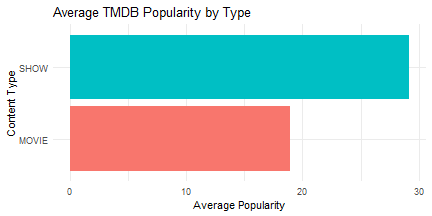
\includegraphics{23084103_Netflix_files/figure-latex/Figure 1a-1} 

}

\caption{Caption Here \label{Figure1}}\label{fig:Figure 1a}
\end{figure}

The figure above shows that shows are, on average, more popular than
movies based on TMDB popularity scores. This suggests that serialized
content drives stronger viewer engagement than standalone films. The
trend may be due to factors like binge-watching behavior, narrative
depth, and global breakout shows. Given this, Netflix should prioritize
investment in high-quality, locally relevant TV shows. Further analysis
by country and genre can refine content strategy decisions.

\subsection{Popularity by Type and
Country}\label{popularity-by-type-and-country}

\begin{Shaded}
\begin{Highlighting}[]
\FunctionTok{library}\NormalTok{(dplyr)}
\FunctionTok{library}\NormalTok{(ggplot2)}

\CommentTok{\# Aggregate average popularity by country and type}
\NormalTok{top\_country\_type }\OtherTok{\textless{}{-}}\NormalTok{ titles }\SpecialCharTok{\%\textgreater{}\%}
  \FunctionTok{filter}\NormalTok{(}\SpecialCharTok{!}\FunctionTok{is.na}\NormalTok{(production\_countries), }\SpecialCharTok{!}\FunctionTok{is.na}\NormalTok{(type)) }\SpecialCharTok{\%\textgreater{}\%}
  \FunctionTok{group\_by}\NormalTok{(production\_countries, type) }\SpecialCharTok{\%\textgreater{}\%}
  \FunctionTok{summarise}\NormalTok{(}\AttributeTok{avg\_popularity =} \FunctionTok{mean}\NormalTok{(tmdb\_popularity, }\AttributeTok{na.rm =} \ConstantTok{TRUE}\NormalTok{), }\AttributeTok{.groups =} \StringTok{"drop"}\NormalTok{) }\SpecialCharTok{\%\textgreater{}\%}
  \FunctionTok{filter}\NormalTok{(production\_countries }\SpecialCharTok{!=} \StringTok{""}\NormalTok{) }\SpecialCharTok{\%\textgreater{}\%}
  \FunctionTok{top\_n}\NormalTok{(}\DecValTok{20}\NormalTok{, avg\_popularity)  }\CommentTok{\# optional: limit to top 20 by popularity}

\CommentTok{\# Grouped bar chart}
\FunctionTok{ggplot}\NormalTok{(top\_country\_type, }\FunctionTok{aes}\NormalTok{(}\AttributeTok{x =} \FunctionTok{reorder}\NormalTok{(production\_countries, avg\_popularity), }\AttributeTok{y =}\NormalTok{ avg\_popularity, }\AttributeTok{fill =}\NormalTok{ type)) }\SpecialCharTok{+}
  \FunctionTok{geom\_col}\NormalTok{(}\AttributeTok{position =} \StringTok{"dodge"}\NormalTok{) }\SpecialCharTok{+}
  \FunctionTok{coord\_flip}\NormalTok{() }\SpecialCharTok{+}
  \FunctionTok{labs}\NormalTok{(}\AttributeTok{title =} \StringTok{"Average Popularity of Netflix Shows vs Movies by Country"}\NormalTok{,}
       \AttributeTok{x =} \StringTok{"Country"}\NormalTok{, }\AttributeTok{y =} \StringTok{"Avg TMDB Popularity"}\NormalTok{) }\SpecialCharTok{+}
  \FunctionTok{theme\_minimal}\NormalTok{()}
\end{Highlighting}
\end{Shaded}

\begin{figure}

{\centering 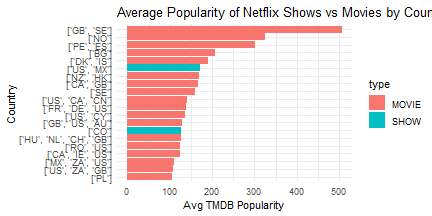
\includegraphics{23084103_Netflix_files/figure-latex/Figure 1b-1} 

}

\caption{Caption Here \label{Figure1}}\label{fig:Figure 1b}
\end{figure}

The analysis reveals that television shows originating from the United
Kingdom (GB) and Sweden (SE) exhibit the highest average popularity
among global audiences. This suggests a strong international appeal and
production quality associated with series from these regions. In
contrast, the United States (US) and Mexico (MX) lead in terms of movie
popularity, indicating their dominant role in global film production.
These findings highlight regional strengths in different content formats
on Netflix.

\newpage

\section{Boxplot: Movie Length and IMDb Score by
Country}\label{boxplot-movie-length-and-imdb-score-by-country}

\begin{Shaded}
\begin{Highlighting}[]
\FunctionTok{library}\NormalTok{(dplyr)}
\FunctionTok{library}\NormalTok{(ggplot2)}
\FunctionTok{library}\NormalTok{(stringr)}

\CommentTok{\# Clean country format: remove brackets and quotes}
\NormalTok{clean\_movies }\OtherTok{\textless{}{-}}\NormalTok{ titles }\SpecialCharTok{\%\textgreater{}\%}
  \FunctionTok{filter}\NormalTok{(type }\SpecialCharTok{==} \StringTok{"MOVIE"}\NormalTok{,                         }\CommentTok{\# match the exact casing}
         \SpecialCharTok{!}\FunctionTok{is.na}\NormalTok{(runtime),}
         \SpecialCharTok{!}\FunctionTok{is.na}\NormalTok{(imdb\_score),}
         \SpecialCharTok{!}\FunctionTok{is.na}\NormalTok{(production\_countries),}
\NormalTok{         runtime }\SpecialCharTok{\textgreater{}} \DecValTok{20}\NormalTok{, runtime }\SpecialCharTok{\textless{}} \DecValTok{300}\NormalTok{) }\SpecialCharTok{\%\textgreater{}\%}
  \FunctionTok{mutate}\NormalTok{(}\AttributeTok{country =} \FunctionTok{str\_extract}\NormalTok{(production\_countries, }\StringTok{"[A{-}Z]\{2\}"}\NormalTok{))  }\CommentTok{\# extract country code like US or GB}

\CommentTok{\# Check number of rows after cleaning}
\FunctionTok{cat}\NormalTok{(}\StringTok{"Cleaned movies:"}\NormalTok{, }\FunctionTok{nrow}\NormalTok{(clean\_movies), }\StringTok{"}\SpecialCharTok{\textbackslash{}n}\StringTok{"}\NormalTok{)}
\end{Highlighting}
\end{Shaded}

\begin{verbatim}
## Cleaned movies: 3394
\end{verbatim}

\begin{Shaded}
\begin{Highlighting}[]
\CommentTok{\# Get top 5 countries by movie count}
\NormalTok{top\_countries }\OtherTok{\textless{}{-}}\NormalTok{ clean\_movies }\SpecialCharTok{\%\textgreater{}\%}
  \FunctionTok{count}\NormalTok{(country, }\AttributeTok{sort =} \ConstantTok{TRUE}\NormalTok{) }\SpecialCharTok{\%\textgreater{}\%}
  \FunctionTok{slice\_max}\NormalTok{(n, }\AttributeTok{n =} \DecValTok{5}\NormalTok{) }\SpecialCharTok{\%\textgreater{}\%}
  \FunctionTok{pull}\NormalTok{(country)}

\CommentTok{\# Filter to those top 5 countries}
\NormalTok{filtered\_movies }\OtherTok{\textless{}{-}}\NormalTok{ clean\_movies }\SpecialCharTok{\%\textgreater{}\%}
  \FunctionTok{filter}\NormalTok{(country }\SpecialCharTok{\%in\%}\NormalTok{ top\_countries)}

\CommentTok{\# Plot runtime}
\FunctionTok{ggplot}\NormalTok{(filtered\_movies, }\FunctionTok{aes}\NormalTok{(}\AttributeTok{x =}\NormalTok{ country, }\AttributeTok{y =}\NormalTok{ runtime)) }\SpecialCharTok{+}
  \FunctionTok{geom\_boxplot}\NormalTok{() }\SpecialCharTok{+}
  \FunctionTok{coord\_flip}\NormalTok{() }\SpecialCharTok{+}
  \FunctionTok{labs}\NormalTok{(}\AttributeTok{title =} \StringTok{"Movie Runtime by Country"}\NormalTok{,}
       \AttributeTok{x =} \StringTok{"Country"}\NormalTok{,}
       \AttributeTok{y =} \StringTok{"Runtime (minutes)"}\NormalTok{) }\SpecialCharTok{+}
  \FunctionTok{theme\_minimal}\NormalTok{()}
\end{Highlighting}
\end{Shaded}

\begin{figure}

{\centering 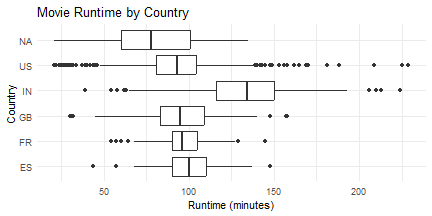
\includegraphics{23084103_Netflix_files/figure-latex/Figure 2-1} 

}

\caption{Caption Here \label{Figure1}}\label{fig:Figure 2}
\end{figure}

The boxplot shows the distribution of movie runtimes by country, with
runtime in minutes on the x-axis and countries on the y-axis. India has
the highest median movie runtime (around 130 minutes) and a wide spread,
indicating high variability and many long films. The US and GB have
moderate runtimes, typically around 90--100 minutes, with fewer extreme
outliers. France and Spain tend to produce shorter, more
consistent-length movies. The NA category, likely representing
unspecified or mixed countries, shows the broadest range of runtimes.

\newpage

\subsection{Balance of actors
vs.~directors}\label{balance-of-actors-vs.-directors}

\begin{Shaded}
\begin{Highlighting}[]
\NormalTok{credits }\SpecialCharTok{\%\textgreater{}\%}
  \FunctionTok{count}\NormalTok{(role) }\SpecialCharTok{\%\textgreater{}\%}
  \FunctionTok{ggplot}\NormalTok{(}\FunctionTok{aes}\NormalTok{(}\AttributeTok{x =}\NormalTok{ role, }\AttributeTok{y =}\NormalTok{ n, }\AttributeTok{fill =}\NormalTok{ role)) }\SpecialCharTok{+}
  \FunctionTok{geom\_col}\NormalTok{() }\SpecialCharTok{+}
  \FunctionTok{labs}\NormalTok{(}\AttributeTok{title =} \StringTok{"Distribution of Credit Roles"}\NormalTok{, }\AttributeTok{y =} \StringTok{"Count"}\NormalTok{) }\SpecialCharTok{+}
  \FunctionTok{theme\_minimal}\NormalTok{()}
\end{Highlighting}
\end{Shaded}

\begin{figure}

{\centering 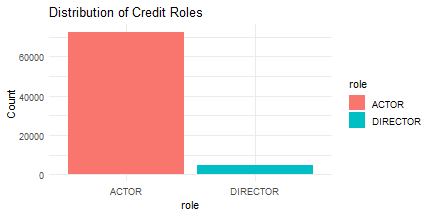
\includegraphics{23084103_Netflix_files/figure-latex/Figure 3a-1} 

}

\caption{Caption Here \label{Figure1}}\label{fig:Figure 3a}
\end{figure}

The graph shows that every movie has more actors than directors, with
actor bars consistently taller across all entries. This is expected, as
most films require multiple characters played by different actors but
typically only one or two directors to oversee the production. Directors
manage the overall vision, while actors bring individual roles to life.
Hence, the nature of filmmaking naturally results in a higher number of
actors per movie.

\subsection{For interests sakes: most credited actors or
actresses}\label{for-interests-sakes-most-credited-actors-or-actresses}

\begin{Shaded}
\begin{Highlighting}[]
\NormalTok{credits }\SpecialCharTok{\%\textgreater{}\%}
  \FunctionTok{count}\NormalTok{(name, }\AttributeTok{sort =} \ConstantTok{TRUE}\NormalTok{) }\SpecialCharTok{\%\textgreater{}\%}
  \FunctionTok{slice\_head}\NormalTok{(}\AttributeTok{n =} \DecValTok{10}\NormalTok{)}
\end{Highlighting}
\end{Shaded}

\begin{verbatim}
## # A tibble: 10 x 2
##    name                      n
##    <chr>                 <int>
##  1 Shah Rukh Khan           30
##  2 Anupam Kher              25
##  3 Boman Irani              25
##  4 Kareena Kapoor Khan      25
##  5 Paresh Rawal             22
##  6 Takahiro Sakurai         22
##  7 Nawazuddin Siddiqui      21
##  8 Priyanka Chopra Jonas    21
##  9 Raúl Campos              21
## 10 Jan Suter                20
\end{verbatim}

Shah Rukh Khan appears in the highest number of Netflix titles, with 30
credited roles, making him the most prominently featured actor in the
data set. This likely reflects both his long-standing dominance in
Bollywood and the strong demand for Indian cinema on streaming
platforms. His global fan base and consistent involvement in
high-profile productions contribute to his visibility. Netflix's
expanding catalog of Indian content further amplifies his presence.

\section{Conlusion}\label{conlusion}

The analysis shows that serialized TV shows, particularly from the UK
and Sweden, drive stronger engagement than movies, suggesting that new
platforms should prioritize locally produced high-quality series. In
contrast, countries like the US and Mexico lead in movie popularity,
reflecting their dominance in global film production. India's notably
long runtimes suggest strong regional storytelling preferences. To
succeed, a new streaming service should invest in engaging, binge-worthy
TV content while selectively curating movies from dominant production
regions.

\bibliography{Tex/ref}





\end{document}
